\section{Gestion de sistemas de información}

\insertsectionpage



\begin{frame}
		
   \frametitle{Importancia de los sistemas de información}

   Para apoyar los procesos misionales en una entidad es importante contar con sistemas de información que permitan:
\begin{columns}
    \begin{column}{.5\textwidth}
      \begin{itemize}	
        \item Habilitar transacciones que generan información.
        \item Garantizar la calidad de los datos.
        \item Proveer información útil para la toma de decisiones.
        \item Facilitar la consulta por grupos de interés.
	\item  Cumplir atributos de calidad.
      \end{itemize}
    \end{column}

    \begin{column}{.5\textwidth}
      \begin{figure}[ht]
        \centering
        
\includegraphics[width=0.7\textwidth]{img/importancia.png}
      \end{figure}
    \end{column}
  \end{columns}

\end{frame}


\begin{frame}

  \frametitle{Gestión de la arquitectura de sistemas de información}

  Documenta y mantiene actualizada la arquitectura de soluciones, manuales y lineamientos técnicos. Esto implica:
  \begin{columns}
    \begin{column}{.5\textwidth}
      \begin{itemize}	
        \item Identificar y caracterizar los sistemas de información.
        \item Entender cómo habilitan procesos y servicios.
        \item Visualizar actores, flujos de información e interoperabilidad.
        \item Tomar decisiones estratégicas para su evolución.
      \end{itemize}
    \end{column}

    \begin{column}{.5\textwidth}
      \begin{figure}[ht]
        \centering
        
\includegraphics[width=0.7\textwidth]{img/arquitectura.jpg}
      \end{figure}
    \end{column}
  \end{columns}


\end{frame} 

\begin{frame}
  \frametitle{Apoyo de los sistemas de información a los procesos}
  \begin{figure}[ht]
     \centering
     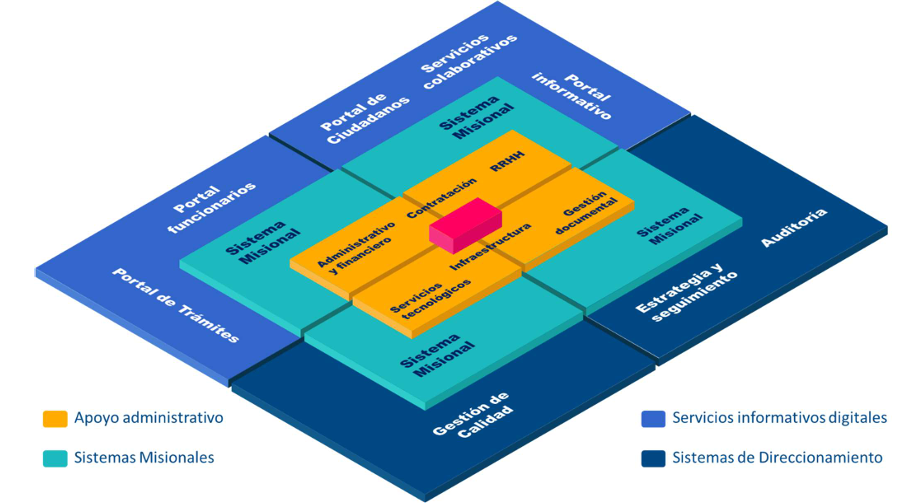
\includegraphics[width=0.7\textwidth]{img/procesos.png}
     \caption{\label{fig:procesos} Estructura general de los sistemas de información, \cite{MinTIC2021marco}}
  \end{figure}
\end{frame}
